\documentclass[sigplan,screen,10pt]{acmart}
\usepackage[utf8]{inputenc}
\usepackage[T1]{fontenc}
\usepackage[french]{babel}

\begin{document}
	\section*{Number of accesses to cluster}
	
	This describe, the number of accesses to a same cluster per snapshot during a workload.
	I focus here on chain of 50 and 500 snapshots.
	We noticed that in vanilla version, the number of accesses if larger because we are always looking for all the pasts snapshots in order to find a specific cluster.
	
	With our direct-access method, we only have the exact number of accesses which give us the real index and then we can jump to that snapshot index, omitting access to intermediate snapshots.
	
	\begin{figure}[h]
		\center
		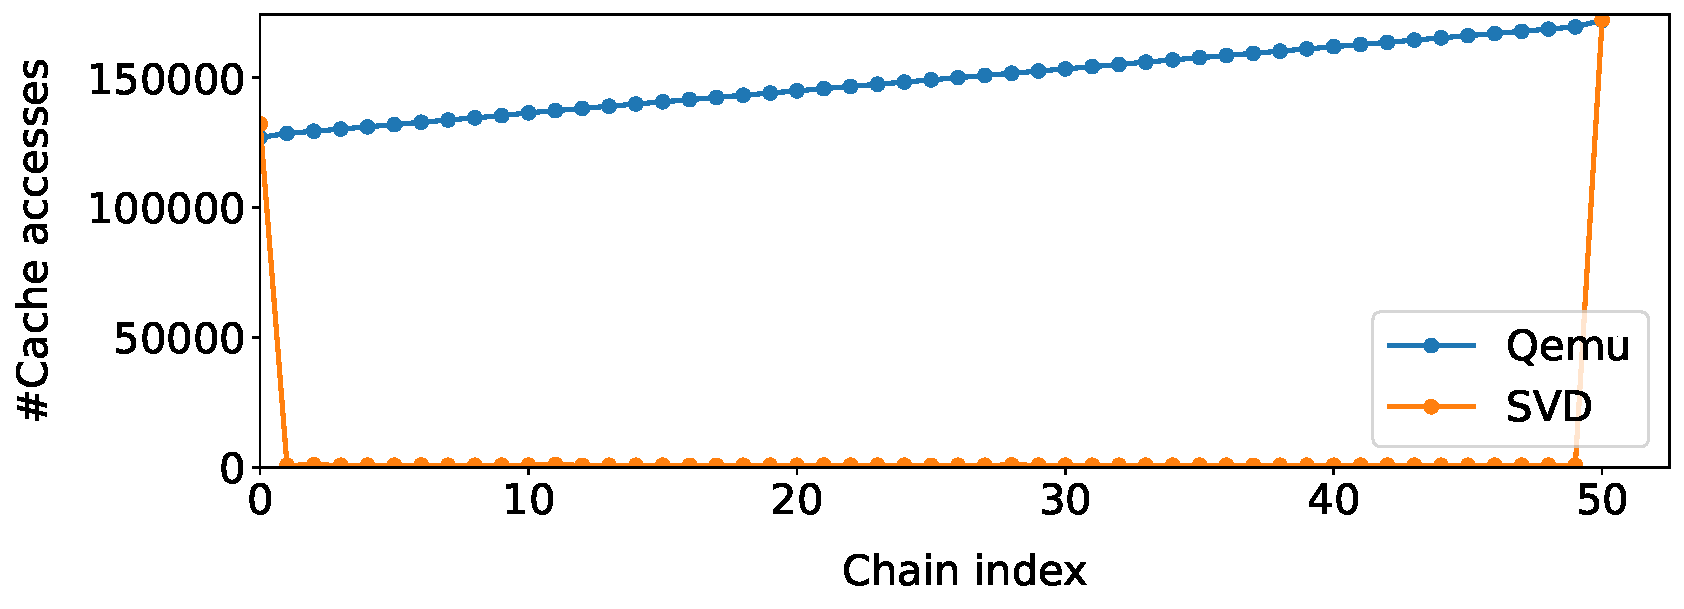
\includegraphics[width=0.45\textwidth]{clusters_accesses_chain_50.pdf}
		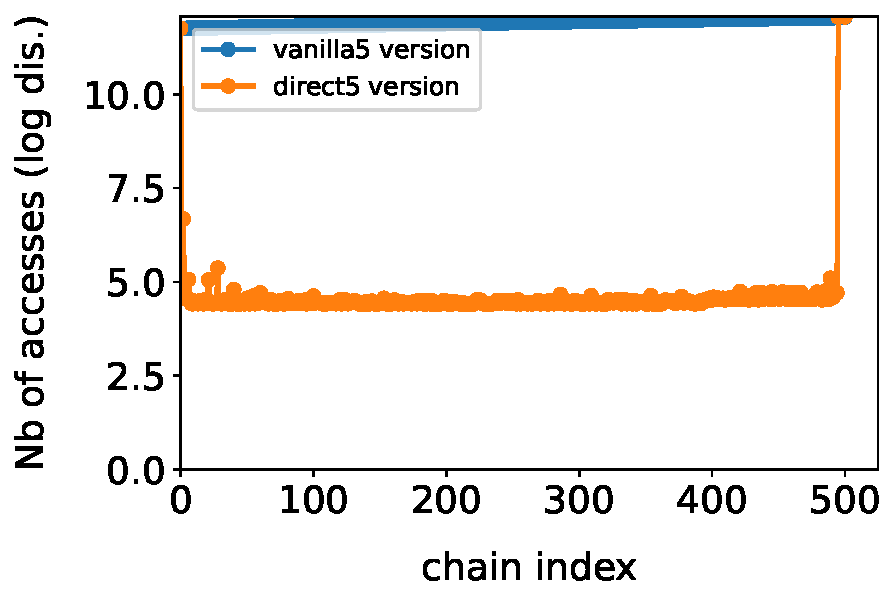
\includegraphics[width=0.45\textwidth]{clusters_accesses_chain_500.pdf}
		\caption{Accesses in a chain of 50 and 500 snap}
		\label{fig:fig2}
	\end{figure}


	\section*{Details on type of accesses to cluster (events)}
	
	Here, we focus on explaining why there are more accesses in vanilla version, and we are doing it by distinguishing all the type of access results (here we call it \textit{event}) in each chain.
	\begin{itemize}
		\item unallocated => the cluster is not allocated in the current snap
		\item normal => the cluster is allocated in the current (occured when we resolve an unallocated event)
		\item hit/missed => relative to the fact that cluster metadata are presented/not presented in the cache
	\end{itemize}
	
	
	\begin{figure}[h]
		\center
		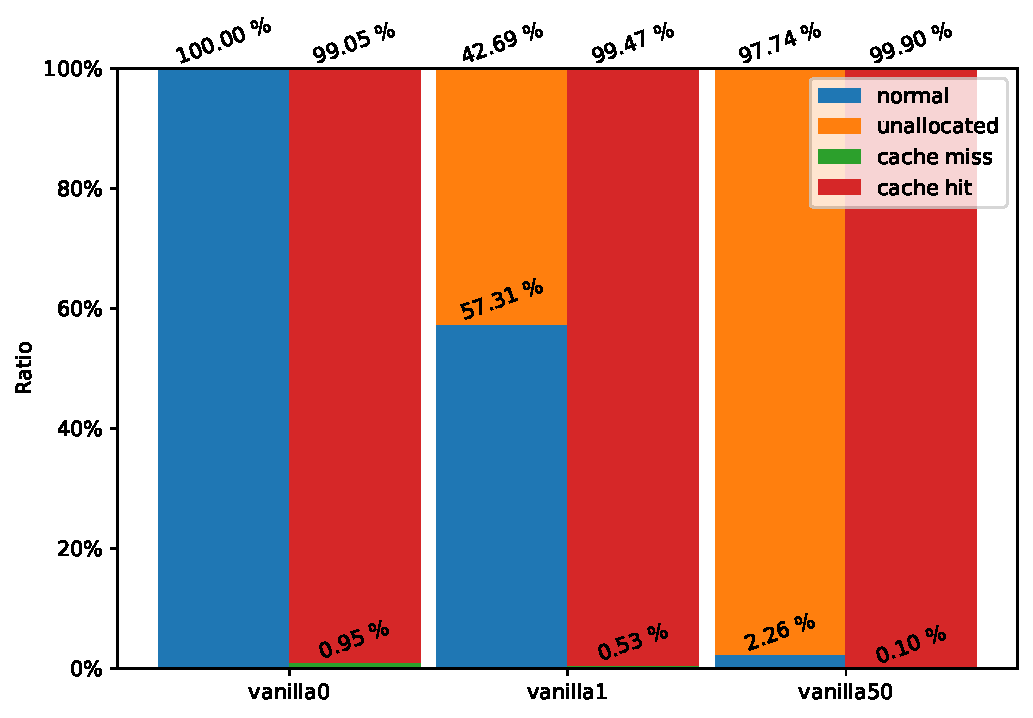
\includegraphics[width=0.6\textwidth]{number_events_per_chain_va.pdf}
		\caption{Number of events (unallocated, missed, hit, normal) for the vanilla version, the number on the x-axis indicate the chain length corresponding}
		\label{fig:fig36}
	\end{figure}

	We noticed that in the vanilla version, the number of unallocated events that we get in order to get the current location of the cluster (normal event occurence) increased exponentially with the chain of the length. While in our direct-access version, we always approximatively have the same number of unallocated and normal event regardless of the chain length, this due to the fact that a same "unallocated event" is not propagate all over the chain like in the vanilla version.
	
	\begin{figure}[h]
		\center
		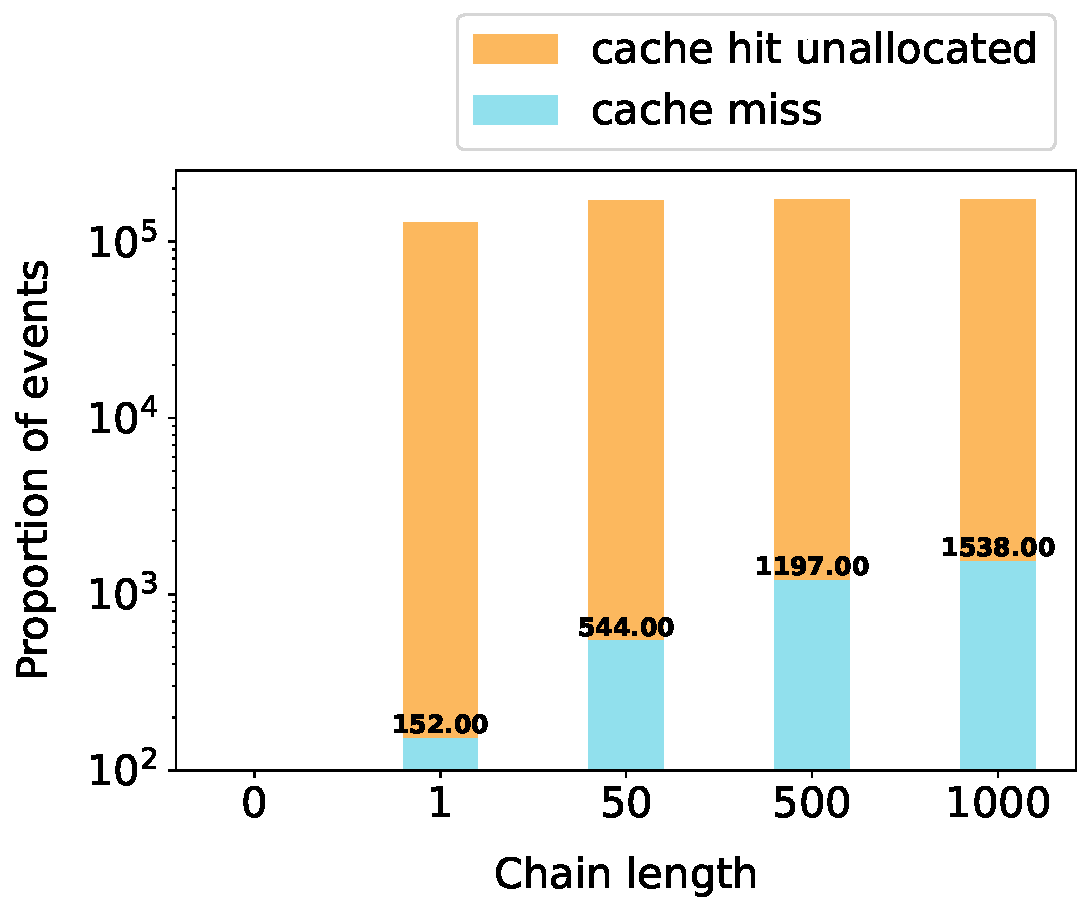
\includegraphics[width=0.6\textwidth]{number_events_per_chain_di.pdf}
		\caption{Number of events (unallocated, missed, hit, normal) in the direct-access version}
		\label{fig:fig37}
	\end{figure}


	\section*{Memory footprint}
	
	Comparison of memory footprint and throughput during workload dd, between our version and the vanilla one.
	
	\begin{figure}[h]
		\center
		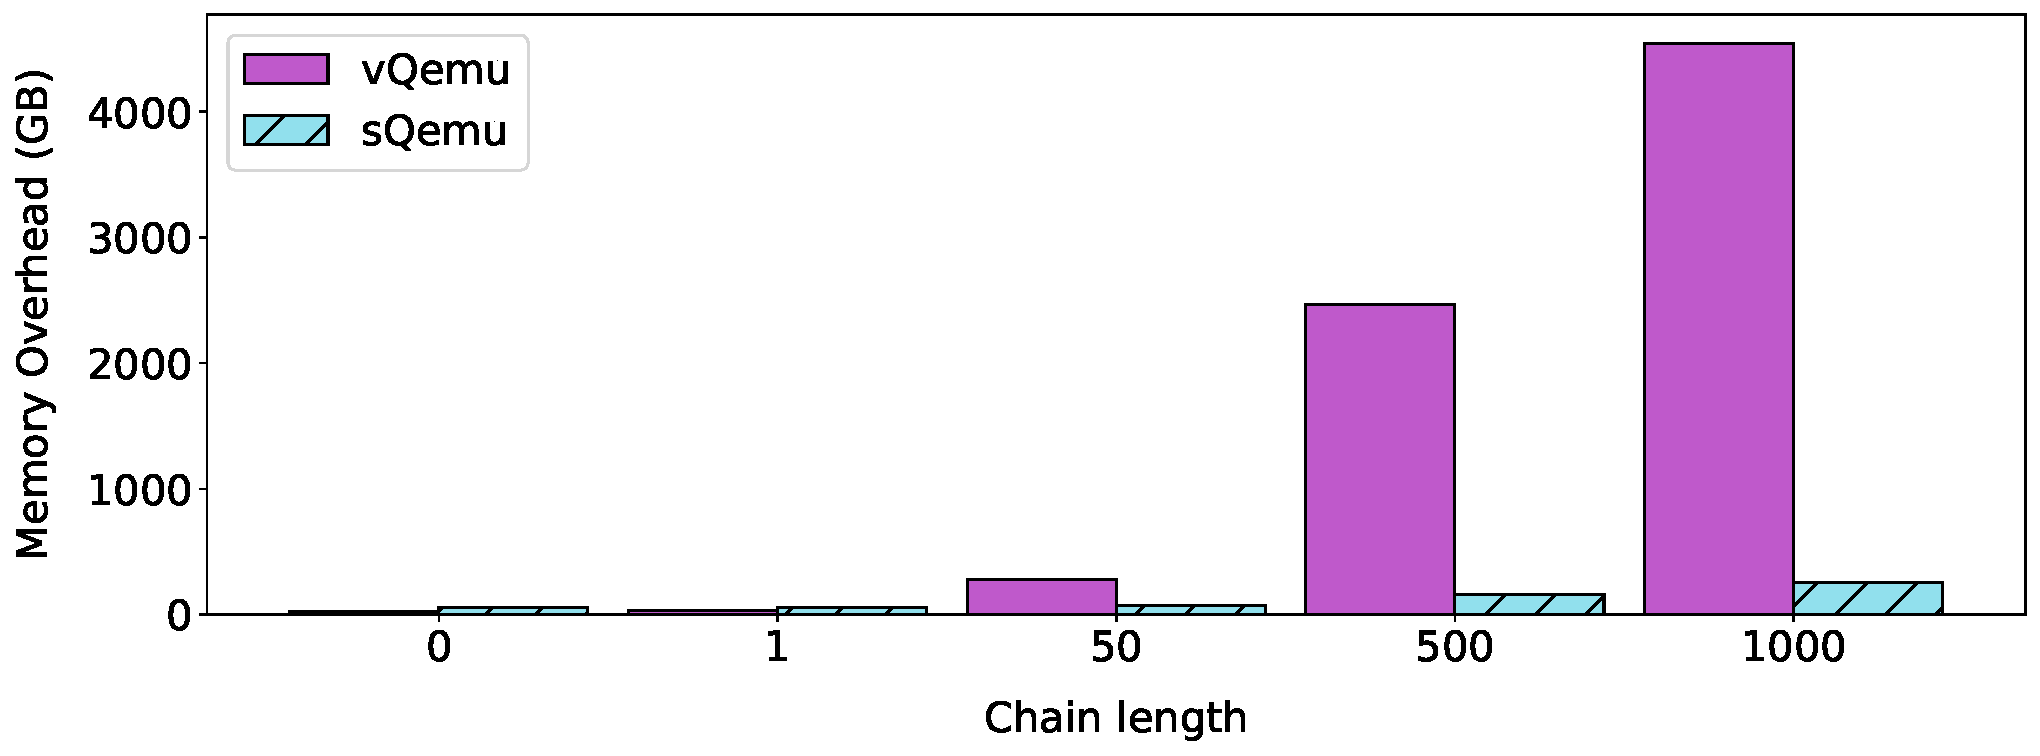
\includegraphics[width=0.45\textwidth]{memory_consumption.pdf}
		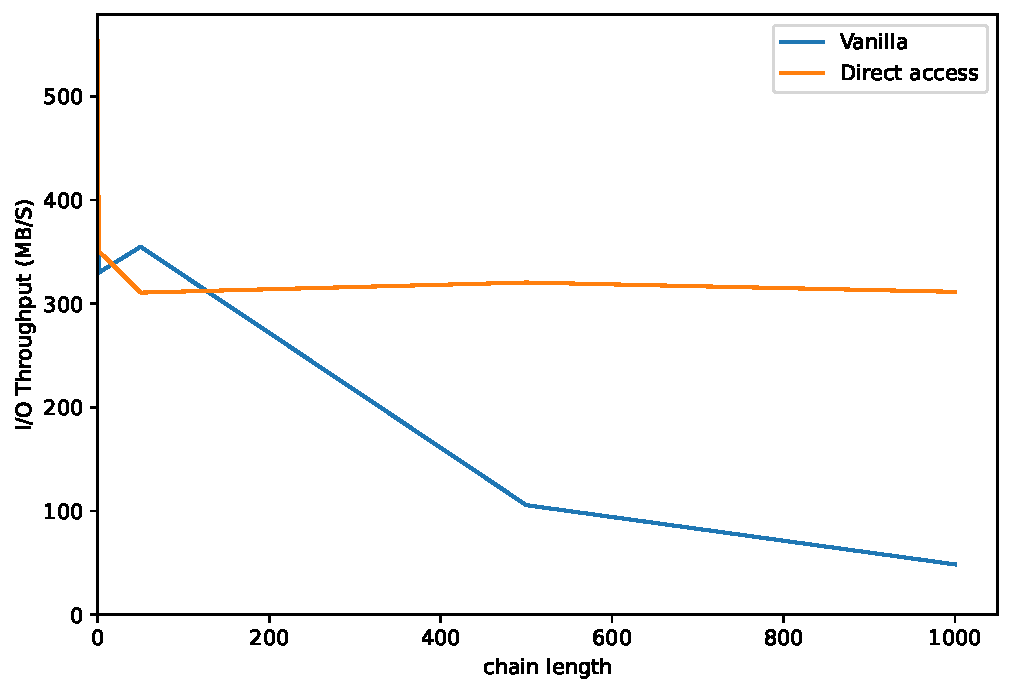
\includegraphics[width=0.45\textwidth]{workload_dd_throughput.pdf}
		\caption{Memory consumption and Throughput (I/O) during all the workload}
		\label{fig:fig3}
	\end{figure}
	
	\section*{Startup duration}
	
	The first evaluation i did, presenting the startup duration of a Virtual machine, comparison between our version and vanilla qemu
	
	\begin{figure}[h]
		\center
		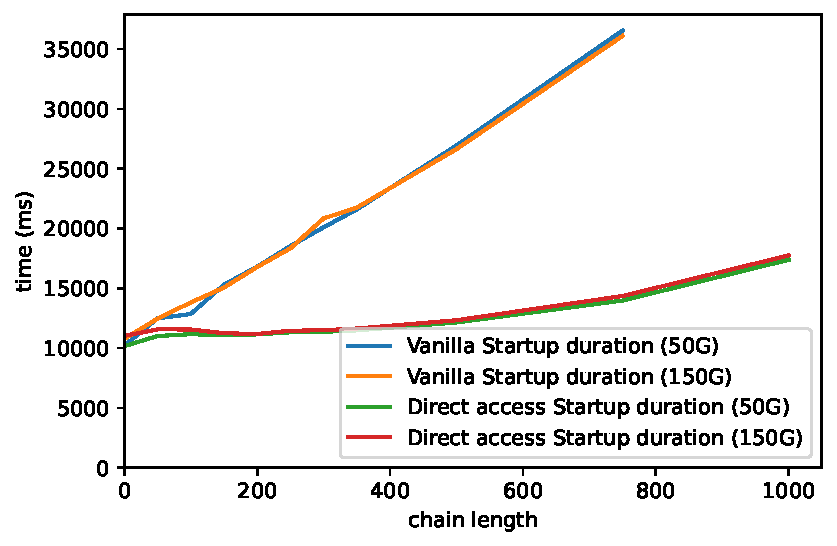
\includegraphics[width=0.45\textwidth]{startup_duration.pdf}
		\caption{Startup, vanilla and direct-access version on 50G and 150G disk}
		\label{fig:fig34}
	\end{figure}

	\section*{Hits and Missed treatment times}
	
	It is important to notice we are always working on chain of snapshots. Here, we call \textit{Cache hit}, all the operations needed by the driver to get access successfully to an l2 entry describing a cluster without going on image file to find it (i.e looking only in memory). And then, \textit{Cache Missed} is when we had to go at least once on image files (important to precise we can go many times on disk to look in the different snapshots image file). We did this on HDD hard disk as used by most of cloud providers, and SSD hard disk, supposing that we are in the best cases of hard disk speed.
	
	\subsection*{Cache Missed treatment times}
	
	\textit{Van/Dir x: Vanilla/Our version run on a chain of x snapshots. \textbf{base} for a chain without snapshots, 1 image}
	\begin{figure}[h]
		\center
		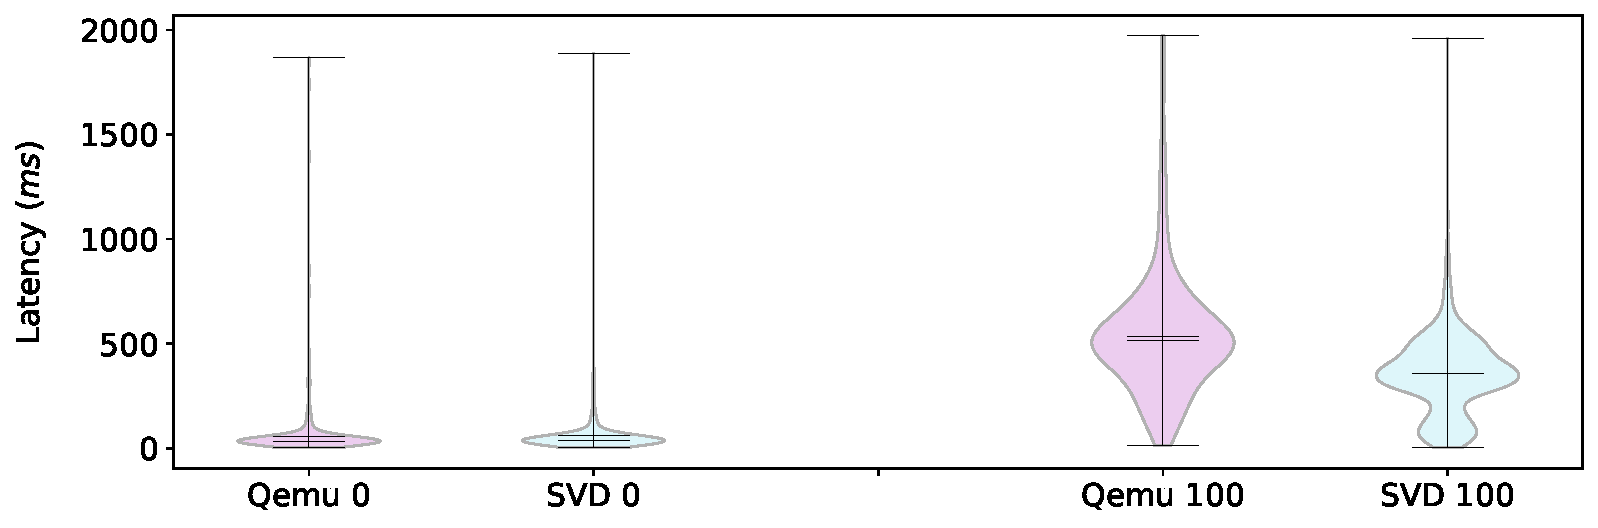
\includegraphics[width=0.45\textwidth]{MISSED_time_hdd.pdf}
		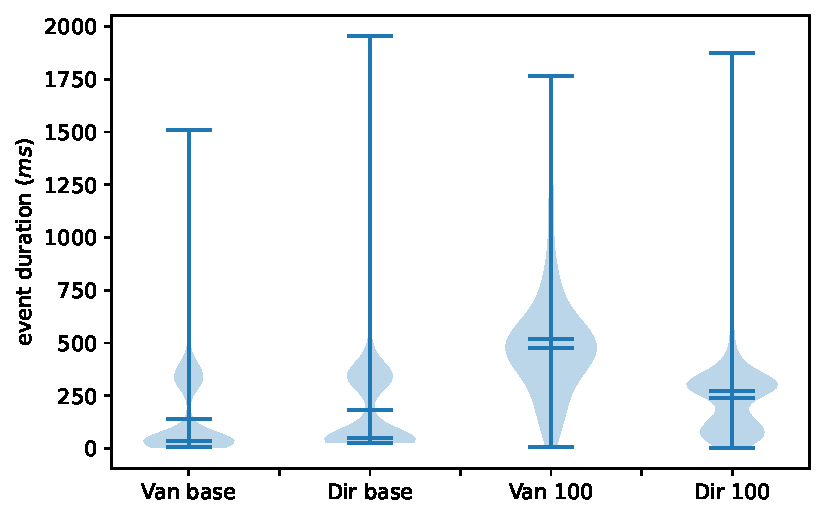
\includegraphics[width=0.45\textwidth]{MISSED_time_ssd.pdf}
		\caption{On the left, boxplot presenting time to resolve cache missed with images file stored on a HDD hard disk. On the right, the same with images file on an SSD hard disk}
		\label{fig:fig-a}
	\end{figure}

	Obviously, when there is no snapshots (Van/Dir base), there are no differences between the 2 version, times of treatment are the same.
	
	However, when the chain length increases, treatment of a cache missed take generally 500ms in vanilla while it take less than ~300ms in our solution and this is for a chain of only 100 snapshots.
	
	Another notice we did was the large repartition of time in vanilla version. This large repartition of time report another problem which is the unpredictability of performance, due to the time which can have a variety of values in this large field of possible values. Our solution try somehow to reduce this large repartition possibility but don't cancel it totally; but it is normal. It's not the goal of our work.
	
	\subsection*{Cache hit times}
	
	\begin{figure}[h]
		\center
		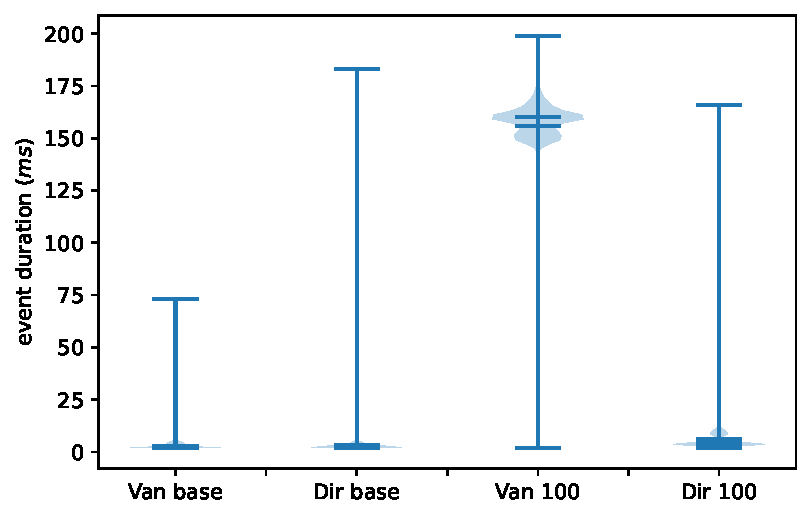
\includegraphics[width=0.45\textwidth]{HIT_time_hdd.pdf}
		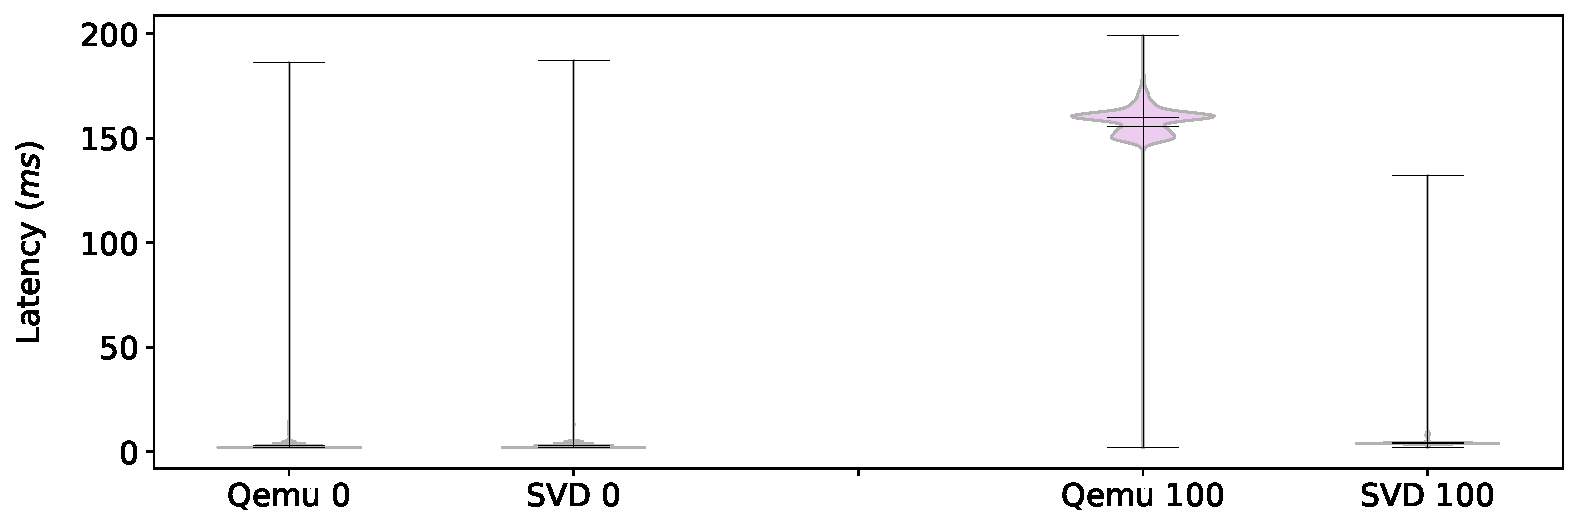
\includegraphics[width=0.45\textwidth]{HIT_time_ssd.pdf}
		\caption{On the left, boxplot presenting time to get value in the cache with images file stored on a HDD hard disk. On the right, the same with images file on an SSD hard disk}
		\label{fig:fig_b}
	\end{figure}

	Nothing to say about chain of 0 snapshot. Hits are often few operations at the order of $\mu$s. So it's normal that times are so small here, either on HDD or SSD hard disk.
	But, when we scale, by using chain of 100 snapshots for example, in vanilla we take too much time because each hit operation knock on all the intermediate caches where in our solution, we only knock on the first cache and the one where the information we are looking is. It is why our times are near the times observed as if there are no snapshots.
	The other notice we can do is that hit times are not affect by the type of hard disk used (HDD/SDD) because all hits are done in memory.
	
	\section*{Comparison of performance - Our solution/Vanilla with cache variation}
	
	Here, we vary the cache parameter for the VM while starting her. And we launch a random workload (fio).
	The goal is to compared our solution and vanilla one when each other use the same amount of cache 
	
	\begin{figure}[h]
		\center
		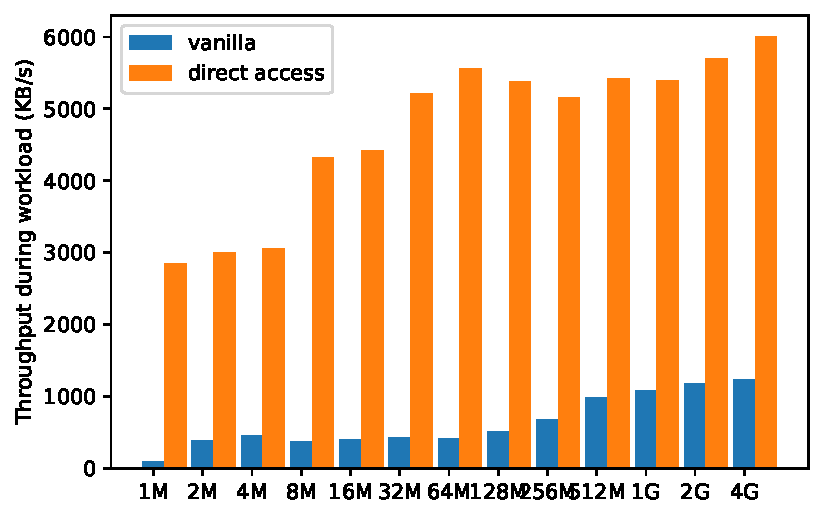
\includegraphics[width=0.45\textwidth]{cache_variation.pdf}
		\caption{Cache variation while running a random read workload on a chain of 500 snapshots}
		\label{fig:fig-c}
	\end{figure}

	Nothing to say here too i guess, our solution is always better; even when the performance of vanilla increases with cache allocated to him that increased, our solution is always better.
	
	The second notice to do here is that after cache size $>$ 4MB, performance didn't vary a lot in our solution. Due to the fact that we only need less than 4MB for this specific disk size and chain length.
	
	\section*{Cache deduplication in Vanilla version}
	
	In order to prove that really exists cache deduplication in vanilla, we did this other evaluation: Counting cluster metadata that were presented many times in the differents cache of each snapshot; then calculate the amount of memory we wasted. The evaluation was did on a chain of 100 snapshots, The cache memory needed to contain all the metadata is 7MB in this case.
	
	This graph presented the amount of memory wasted (duplication) during a workload (fio random read) from the startup of the VM to his shutdown.
	
	\begin{figure}[h]
		\center
		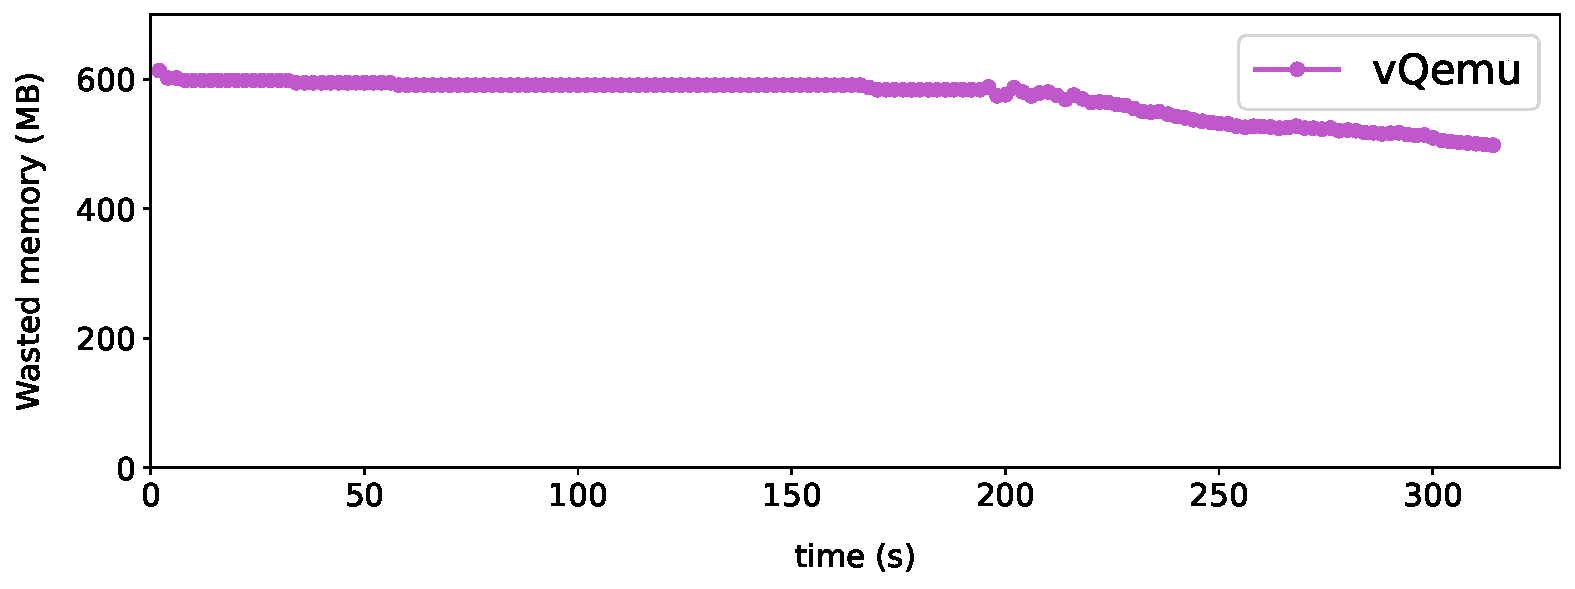
\includegraphics[width=0.45\textwidth]{dupli_memory.pdf}
		\caption{Startup, vanilla and direct-access version on 50G and 150G disk}
		\label{fig:fig-d}
	\end{figure}

\end{document}